\section{\normalsize Диаграмма фазового равновесия «твёрдое тело--жидкость--пар». Тройная точка.}
\paragraph{Диаграмма фазового равновесия «твёрдое тело--жидкость--пар».}$\;$\\
\begin{minipage}{75mm}
	\begin{figure}[H]
		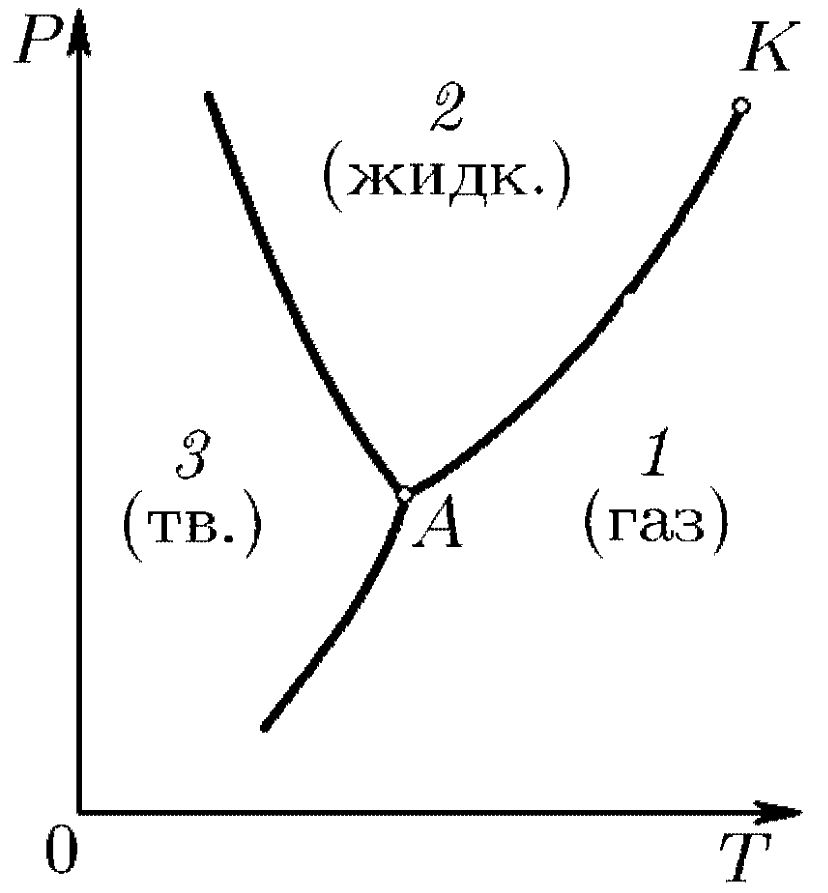
\includegraphics[width=65mm]{ris17.png}
	\end{figure}
\end{minipage}
\begin{minipage}{100mm}
	Рассмотрим трех фазную систему. Для равновесия необходимо:
	\begin{enumerate}[(1)]
		\item $\varphi_1(P,T)=\varphi_2(P,T)$ --- кривая испарения 12
		\item $\varphi_2(P,T)=\varphi_3(P,T)$ --- кривая плавления 23
		\item $\varphi_1(P,T)=\varphi_3(P,T)$ --- кривая возгонки 31
	\end{enumerate}
	Все они пересекаются в т.А
\end{minipage}
\paragraph{Тройная точка.}
Точка А называется \textbf{тройной точкой}, три фазы могут находится в равновесии друг с другом, лишь в этой точке, имеющей конкретный параметры. В малой окрестности тройной точки можно провести круговой изотермический процесс, для которого справедливо
$$\oint\dfrac{\delta Q}{T}=0\underset{T=const}{\longmapsto}\oint\delta Q \Rightarrow q_\text{13}=q_\text{32}+q_\text{21}$$
